\documentclass{article}
\usepackage[utf8]{inputenc}
\usepackage[margin=0.75in]{geometry}
\usepackage{graphicx}
\begin{document}
	\begin{center}
    
    	% MAKE SURE YOU TAKE OUT THE SQUARE BRACKETS
    
		\LARGE{\textbf{IDEA PROPOSAL}} \\
        \vspace{1em}
        \LARGE{\textbf{e-Yantra Ideas Competition}} \\
        \vspace{1em}
        \Large\textbf{Team ID: 118} \\
        \vspace{1em}
        \normalsize\textbf{Govintha Raj K} \\
        \normalsize\textbf{Kavinraja G} \\
        \normalsize\textbf{Heeraj A} \\
        \normalsize\textbf{Anand A T} \\
        \vspace{1em}
        \normalsize\textbf{Mentor: Mr. V. Arunkumar} \\
        \normalsize{Department of Mechatronics Engineering} \\
        \normalsize{Kongu Engineering College, Erode}
     
	\end{center}
	\begin{normalsize}
		\section*{Project Name:}
		 {\large Flying Quadruped Robot for Surveillance and Exploration}
	\end{normalsize}
    \begin{normalsize}
    
    	\section*{Introduction:}
        
        Walking robots mostly have advantages over other types of locomotion. They can move on unstructured terrains that are too difficult for conventional robots. They are highly stable and carry greater loads. They are also used to create detailed 3D maps of the environment and to find people who may be trapped in disaster zones .The defense of any country involves conducting basic surveys of potentially hazardous areas to ensure protection of the people and the place . Using drones reduces manual labour and can obtain a greater field of view. This also does not risks the lives of the people as they do not have to enter these dangerous areas. By using walking drones we can ensure the advantage of both walking and flying robots.   \\
      
		\section*{Market Research:}
        
       Existing survival drones are DJI Phantom 4[1], Parrot Bebop 2[2], Yuneec Typhoon Q500[3]. They are explicitly made for Obstacle Avoidance, Active Track, higher speeds and longer flight times. Existing quad pods are Dr . Robot Jaguar Lite Tracked Mobile Platform[4], Rover Robotics[5] are designed to move on unstructured terrains. Our project comprises of both legged system and drones.\\
        
	   	\section*{Approach:}
        
      A typical unmanned aircraft is made of light composite materials to reduce weight and increase maneuverability. This composite material strength allows military drones to cruise at extremely high altitudes. Drones are equipped with different state of the art technology such as infrared cameras, GPS and laser (consumer, commercial and military UAV). Drones are controlled by remote ground control systems (GSC) and also referred to as a ground cockpit. The engineering materials used to build the project are highly complex composites designed to absorb vibration, which decrease the sound produced. These materials are very light weight.  \\
      Our project has three parts, the drone , four legged system and the control system. The four legged system comprises of 3D printed parts. The material used in 3D printing is PLA(Poly Lactic Acid). Each leg has two links providing it a two degrees of freedom. Servo motors are used to achieve movement of the links. Arduino mega is used to control the servo motors .By controlling the links movement individually the robot can be moved. Four legs are attached to a common base. In that base four wings are attached . In each wing a brushless DC motor and a propeller is attached Quadcopters make use of 4 Motors. Two of these motor spin clockwise while the other two spin counter clockwise. Motors on the same axis spin in the same direction.  A quadcopter can either hover or adjust its altitude by applying equal thrust to all four rotors. To adjust its yaw, or make it turn left or right, the quadcopter applies more thrust to one set of motors. Pitch and roll on the other hand are adjusted by apply more thrust on one rotor and less to the other opposing rotor. The device that controls the Brushless DC motors is called an Electronic Speed Controller or ESC. By using controller the desired position can be obtained. By using high definition cameras and sensors the required data can be obtained which can be processed for certain applications. \\
        
    	\section*{Hardware Requirements:}
        \begin{itemize}
        
\item 3D printed links
\item Servo motors
\item Servo Controller
\item The Arduino mega 2560
\item APM-2.8 Flight Controller
\item Brush-less DC motor
\item RF Transmitter and Receiver
\item Lithium polymer Battery

        \end{itemize}
      
		\section*{Software Requirements:}
        \begin{itemize}
		\item Solidworks 2018 
		\item Mission planner
		\item APM planner
		\item Arduino IDE
        \end{itemize}
    	
    	\section*{Flow Chart}
   
\begin{figure}[h!]
	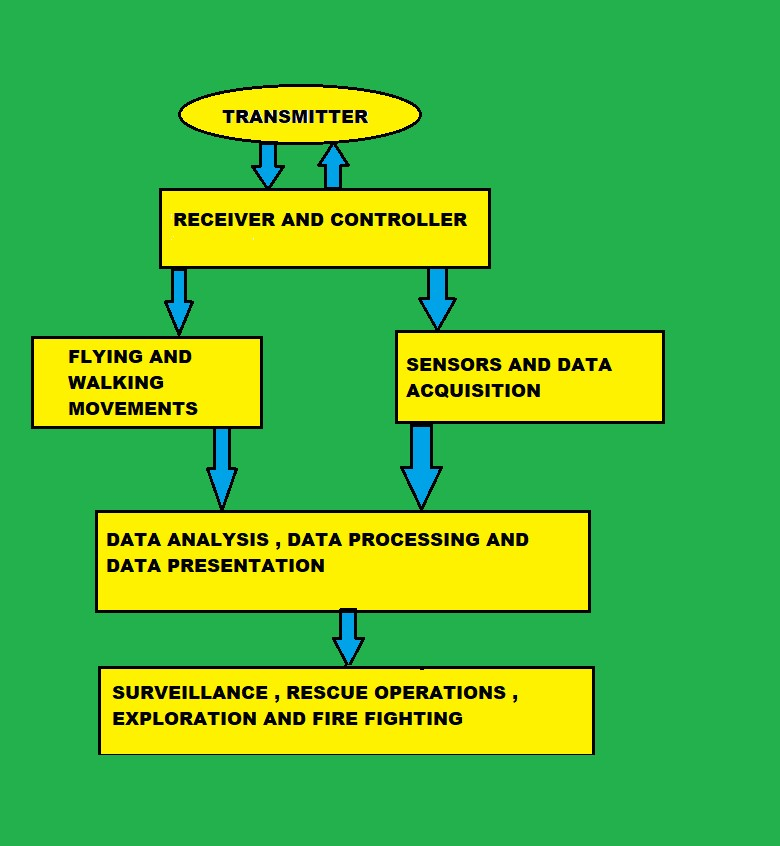
\includegraphics[width=0.4\textwidth]{flow}
	\centering
\end{figure}

    
    	\section*{Feasibility and Future Implementation:}
        Our project overcomes a disadvantage of drone that is unable to move on the land. Though implement of legs increases the weight slightly ,it provides the advantage of more operating time (i.e: it consumes less energy for walking). Our project was designed in phase to increase stability and to obtain precise movement . The implement of legs and cameras makes sure that it can be used effectively for rescue operations. The thermal sensors can be implemented for detection of people .For certain applications pre determined path can be programmed. The controller is user friendly so that it can be controlled at ease.
        
        \section*{References:}
        \begin{enumerate}
        	\item DJI Phantom 4
        	\item Parrot Bebop 2 
            \item Yuneec Typhoon Q500 
           	\item Dr. Robot Jaguar Lite Tracked Mobile Platform 
        	\item Rover Robotics
        \end{enumerate}
\end{normalsize}

  
\end{document}
